\chapter{Related Work}
Enabling simulated movement in virtual environments is not a new problem. 
The techniques that allow the user to move their viewpoint require special attention in regards to immersiveness, cybersickness, ergonomics and path integration, concepts explained in the following chapter.

\section{Motion Sickness}\label{motion-sickness}

The phenomenon, known today as motion sickness, predates modern technology
by millennia, and even Hippocrates wrote about it. The word ``nausea'',
the main symptom of motion sickness, is also derived from the Greek word
for ship ``naus''. \cite{Golding} It is a very
unpleasant feeling and was even used as a legal punishment in the 19th
Century \cite{Reason}. The source of motion sickness is
well understood because there is a lot of research from military agencies
since they had to transport a lot of soldiers by ship and needed them to
be healthy when they reached their destination
\cite{Johnson}. After the invention of the first flight
simulator, the term simulator sickness was coined. Simulator sickness is
a form of motion sickness that can occur when training pilots in
simulators \cite{Johnson}. With the rise of head-mounted
displays and VR technology, motion sickness got another subcategory:
virtual reality sickness, also known as cybersickness. It is distinct
from simulator sickness because the symptoms are not as much related to
the Oculomotor system (for example, eye strain, blurred vision, etc.) but
rather disorienting. The severity was found to be about three times greater
than simulator sickness. This might be because the VR systems are more
immersive than a flight simulator that relies on traditional displays
\cite{Stanney}.\\Because cybersickness and simulator
sickness are different, there needs to be a separate evaluation method
for the two phenomena. According to Stone et al. \cite{Stone}, this is because the
weighted scale of the simulator sickness questionnaire does not
translate well to the VR environment. This is improved with a new
weighting scale proposed by Stone et al. \cite{Stone}, but a new questionnaire
specifically created for cybersickness generates the best results.
However, the simulator sickness questionnaire is often used in reached
anyway. This only has the benefit that the results are easy to compare, but there are significant tradeoffs in regards to accuracy.

\subsection{Cybersickness}\label{cybersickness}

As discussed before, cybersickness is a form of motion sickness. It can
result in a range of symptoms including nausea, vomiting,
disorientation, headaches and eye strain
\cite{LaViola}. This is a serious problem and needs to
be taken into account when developing VR systems.

The actual cause of cybersickness is not known. According to Davis et al. \cite{Davis} the three most prominent theories for the cause of cybersickness are poison theory, postural instability theory and sensory conflict theory.

\begin{itemize}
\itemsep1pt\parskip0pt\parsep0pt
\item
  Poison theory: survival mechanism that induces vomiting and nausea to
  remove poison from the body if the brain detects sensory input like
  hallucinations.\\
\item
  Postural instability theory: a loss of postural control causes
  sickness\\
\item
  Sensory conflict theory: symptoms are created if there is a conflict
  between the vestibular and visual senses. For example, if a user is not
  moving but their avatar in VR is.
\end{itemize}

Unfortunately, all three theories have low predictive power and fail to
explain some key aspects of cybersickness~\cite{Davis}.

One way to reduce cybersickness is to break the optical flow of the user
perceives using different kinds of techniques
\cite{Bhandari}. Optical flow is a phenomenon that
allows an observer to gather information about the motion of objects and
give the observer a sense of presence \cite{Gibson}.

\section{Locomotion in VR}\label{locomotion-in-vr}
The ability to move the players' avatar in the virtual environment is
called locomotion. It is required for many applications or games that
take place on a larger scale. Without locomotion techniques, VR would be
very inaccessible. A user would need a giant tracking space, which is
not possible in most homes and also, the technology to track the user's
headset would have to work accurately over that amount of space. Locomotion is also
needed even if you could walk everywhere in your space since it can
also be a convenience or accessibility feature in combination with a
seated experience. Getting the locomotion mechanics just right will
also improve other interactions and user satisfaction in general. Moving
to a different virtual altitude would also not be possible without some
technique that can simulate the player walking upstairs. Otherwise,
every user would have to have stairs in their tracked space. The
implementations of locomotion techniques can be very diverse, and so there
is a wide range of categorization schemes.

Luca et al. \cite{Luca} collected 109 different locomotion techniques from academic
sources, social media and popular VR games. The result is a public
database of methods that can be filtered and compared. Some of the
methods are in a preliminary state and not fully implemented or
evaluated, but in general, the database is a great resource. There are only eight results for hand-tracking
and some of them falsely categorized.

\subsection{Locomotion using controllers}\label{locomotion-using-controllers}

Boletsis et al. \cite{Boletsis} categorized the four
prevalent locomotion techniques into:

\begin{itemize}
\itemsep1pt\parskip0pt\parsep0pt
\item
  Room-scale-based: uses physical movement, translates movement from the
  real world one to one into VR. Continuos movement, unlimited range.\\
\item
  Motion-based: uses physical movement, for example, swinging arms or
  walking in place. Continuos movement, unlimited range\\
\item
  Controller-based: The uses controller input like a joystick to move.
  Continuos movement, unlimited range.\\
\item
  Teleportation-based: the viewpoint is instantly moved to a new
  predefined location. Non-continuos, unlimited range
\end{itemize}

The room-scale-based techniques are limited to the size of the tracking
space, so they are not flexible enough for a general use case. If the
the task allows, it should be the preferred locomotion technique
because it results in the best immersion while also keeping
cybersickness to a minimum.

Controller-based techniques could be adapted into a hand-tracking
environment, the continuous nature of the movement, without some kind of
a physical representation of the movement performed by the user, however
would make it prone to create motion sickness.

Motion-based techniques are very dynamic because of their physical
nature. That makes them hard to track with current hand-tracking
technology since the hands are often moved quickly and behind the body, outside the tracking area. They also made users tired the fastest.

For those reasons, the scope of this work will focus on only
teleportation-based techniques to give results that are as widely useable as
possible and accessible to the most amount of people without inducing
cybersickness.

\subsubsection{Teleportation-based locomotion}\label{teleportation-based-locomotion}

Teleportation is one of the most used locomotion techniques. Each
implementation can be slightly different in the way it is integrated
into the virtual environment, but the core mechanic allows the user to
move the viewpoint to points on the map using some ray casting system.
There is usually a limit to the teleport distance, and sometimes, the user
is only allowed to select predefined locations as targets. The technique
is categorized as a non-continuous movement with unlimited range. Since not
only the XY coordinates of a target location can be chosen but also
points at different altitudes, the method has 3 degrees of freedom. In some implementations, the viewpoint direction after the teleport can be chosen by the user before the teleport, so they do not have to rotate themselves after the teleport if they prefer to. This gives the user even more control but might be overwhelming for beginners.

The research from Clifton et al. \cite{Clifton} shows that, on average, teleportation
causes less cybersickness than continuous navigation. However, there were
some people (38\%) that had the opposite reaction.
Clifton et al. conclude that there should always be multiple locomotions
methods to choose from. The researchers theorize that the cause of the
cybersickness might be that some people are more sensitive to the
immediate displacement used by teleportation-based locomotion. If the
participants experienced the virtual environment while sitting or
standing did not make a cause a meaningful change in the reported
effects, only that there seems to be slightly worse cybersickness from a
seated experience. 

However, teleportation is also not the perfect solution. 
The lack of optical flow between locations is great to minimize
cybersickness, but it also introduces limitations. 
Path integration is a process where the brain updates the current position
continuously, using information from different senses. Visual, vestibular
and proprioceptive sensory inputs are continuously integrated and create
a rough estimate of the distance travelled. \cite{Bhandari}

Bhandari et al. \cite{Bhandari} found that this can be improved by allowing some optical
flow between teleport points without creating higher levels of
cybersickness. This can be achieved by using a technique the researchers
call ``Dash''. It translates the user at a constant velocity from the
current point to the target. This creates a short transition period that
takes a maximum of 1.1 seconds over a maximum distance of 11 meters in a
virtual environment on a real-world scale. Previous research indicates
that the duration and speed do not impact the resulting effect a lot
\cite{Bowman} but these values were picked after some
internal testing. Using this technique, users were able to move back to
a starting point after teleporting away much more accurately without any
landmark or context clues. 

An interesting problem with teleportation-based locomotion is that it is
found to be the least immersive technique out of the four types
categorized by Boletsis et al. \cite{Boletsis}. This
could improve using hand-tracking because the users can use their own
hands, and that might be more immersive for some people.


\subsection{Locomotion using hand-tracking}\label{locomotion-using-hand-tracking}

Only a rather limited amount of research was done about locomotion using hand-tracking, even though natural human-computer interaction using gestures is not a new field of study. Schäfer et al. \cite{Schafer2021} conducted a study using very basic gestures. In their virtual environment, the simplest gesture only requires the user to point a finger in a forward direction to produce a visual ray in the respective direction. If this ray intersects with a valid teleportation location, a little reticle appears on that point. This marks the teleportation target. If the user keeps their hand still for 1.5s, the teleportation to the target location is performed. Schäfer et al. also implemented other variations on this gesture:

There are two ways to select a location:
\begin{itemize}
  \item point index finger to select a location, named the index method
  \item use the normal vector of the palm to select a location, named the palm method
\end{itemize}

There are also two ways to confirm a target:
\begin{itemize}
  \item the user keeps their hand still for 1.5s
  \item the user uses a second hand to confirm the location. For this, a method was implemented where the left hand can first rest in a neutral position while a target is selected with the right hand. To confirm the teleport location, the user performs a pointing gesture with the second hand while keeping the right hand on the target.
\end{itemize}

The results of a user study conducted by Schäfer et al. \cite{Schafer2021} shows the method using a one-handed palm gesture achieved the highest user satisfaction ratings (90 of 100 possible points). However, there appear to be some problems with the implementation. The authors noticed that bimanual methods lose tracking more often, so this might influence the immersion and user satisfaction results. Another tracking issue was also found with the index method. The noise in the tracking data appears to frustrate users when trying to select a target. The tracking issues make it seem like the one-handed palm gesture was only preferred by users because users found the unreliable tracking frustrating. This is also confirmed by the NASA-TLX results. The users reported being more frustrated with the methods influenced by the bimanual tracking issues and the index finger tracking noise. The method influenced by both types of issues got the worst score. 

\begin{figure}[hbt!]
  \centering
  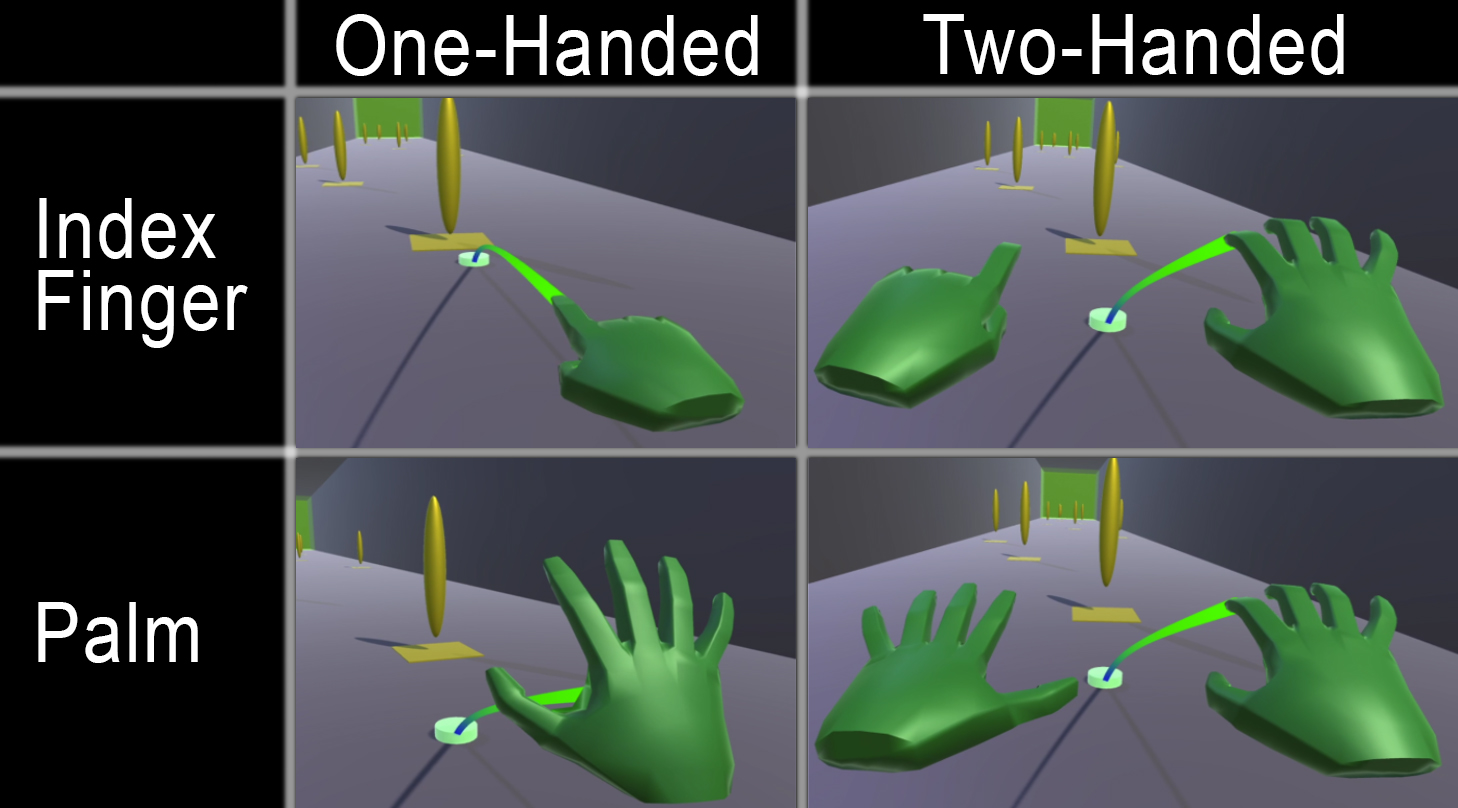
\includegraphics[width=\textwidth]{figures/1h vs 2h gesture study.jpg}
  \caption{Gesture types included in the study from Schäfer et al. \cite{Schafer2021}}
  \label{fig:1vs2}
\end{figure}

The one-handed palm method was the gesture that had the least amount of tracking issues since it was single-handed and was not only using the index finger for target selection. This result is surprising since the gesture violates multiple principles for a comfortable gesture detailed in \ref{ergonomics}. However, in a short study, this might not influence user satisfaction too much. The negative effects of uncomfortable gestures might not be noticeable after only using the gesture for the short duration of the study, so the users are not experiencing the longer-term effects. 

The one-handed palm method, the gesture with the highest usability score, also has other limitations. It would get even more uncomfortable when trying to teleport to some elevated targets. This would put a lot of strain on the wrist, which is one of the most problematic areas. The automatic confirmation of a target used also does not provide any feedback to the user as the bimanual methods do. Some of these issues can be improved on, but it seems like the tracking is the most important issue to solve for now and that this can only be solved using different gestures that enable more robust tracking with less noise.



Another study was performed by Caggianese et al. \cite{Caggianese}. The researchers designed three gesture-based continuous locomotion systems and compared them to a controller-based continuous navigation method. All the gesture-based systems use an activation gesture to prevent accidentally triggering movement while completing other tasks.

The gesture-based techniques are detailed below.

The palm-steering technique (figure \ref{fig:palm}) uses the normal vector of the hand palm plane to set a target point. At this point, it is locked if the user closes their hand. This also starts the movement towards the target. The palm-steering technique allows movement in all directions without the user turning.
\begin{figure}[hbt!]
  \centering
  \includegraphics[width=\textwidth]{figures/palm-gesture.png}
  \caption{Selecting a target using the palm, move to the selected point by closing hand}
  \label{fig:palm}
\end{figure}


The index-steering technique (figure \ref{fig:index}) uses a ray cast from the headset through the position of the tip of the index finger to set the target position. To start the movement, the user moves their thumb in to touch the middle finger.

\begin{figure}[hbt!]
  \centering
  \includegraphics[width=\textwidth]{figures/index-gesture.png}
  \caption{Selecting a target using the index finger, close thumb to start movement}
  \label{fig:index}
\end{figure}


The gaze-steering technique (figure \ref{fig:gaze}) uses only the gaze direction of the headset and a similar technique to the palm-steering technique to start the movement where the user closes their hand.
\begin{figure}[hbt!]
  \centering
  \includegraphics[width=\textwidth]{figures/gaze-gesture.png}
  \caption{Selecting a target using the gaze direction, move to the selected point by closing hand}
  \label{fig:gaze}
\end{figure}

All methods use a targeting system but do not lock the target to a position when the locomotion starts. This led to reports of users preferring the gaze-steering technique since it is the only technique where the hand position does not need to be continuously checked throughout the movement.

The results show that the performance of the gesture-based techniques is similar to the controller locomotion. They do, however, achieve less precision so that users make more errors along the path, and the systems are therefore perceived as more difficult. 

The index-steering technique was praised for the pointing system that is reminiscent of a traditional two-dimensional input system. Also, having different methods for the direction and the movement control is reported to result in higher usability and less physical demand. 



For traditional locomotion using controllers, the locomotion database from Luca et al. \cite{Luca} is a great resource. It includes solutions that are user-tested and established in the industry, as well as more experimental ones. However, when filtering the locomotion database for techniques that are categorized to use hand-tracking, only eight results are presented.
The results that are relevant for this paper are:

\begin{itemize}
\item
  Hand Close: a gesture for a continuous movement that uses the flexing and extending of the fingers as input, as seen in figure \ref{fig:handclose}. Flexed fingers make the user move forward, while extended fingers move the user backwards, with a dead zone in the middle where the fingers can rest. This method seems to have problems
  with producing cybersickness (25\% of the study participants had to abort the 90-minute test). \cite{Huang}
  \begin{figure}[hbt!]
    \centering
    \includegraphics[width=0.6\textwidth]{figures/HUANG gesture.png}
    \caption{Visualization of locomotion control gesture developed by Huang et al. \cite{Huang}}
    \label{fig:handclose}
  \end{figure}

\item
  Finger Run: interesting idea for a two-handed gesture for continuous movement, the only
  resource is a video on a game development account that mostly posts fun
  prototyping ideas \cite{Beauchamp}. The user holds one hand as a flat running surface and forms legs with the index and middle finger of the other hand that walk on the surface of the other hand as seen in figure \ref{fig:fingerrun}. This gesture could not be reproduced with the Meta Quest 2 headsets hand tracking since there was too much occlusion of the lower hand by the upper hand, so the tracking cut out. This could be worked around by guessing the lower hand's position if the tracking cuts out since the hand would get tracked again if the position changes, but this is not a great solution.
  \begin{figure}[hbt!]
    \centering
    \includegraphics[width=0.6\textwidth]{figures/fingerrun.png}
    \caption{Finger run gesture as shown in the demo video \cite{Beauchamp}}
    \label{fig:fingerrun}
  \end{figure}

\item
  Walking stick: a gesture instantiates a walking stick that can be
  used to move the user in relation to the stick's touchpoint on the
  ground. This is only a preliminary database entry, though, and this is
  not a great solution for big distances or different altitudes. The author also included other mechanics that also used the walking stick, for example, a shield or a gun. So this could be a useful method if there are already a number of gadgets present in the environment, and a walking stick would make sense as an addition. \cite{walkingstick}
\end{itemize}

The categorizations seem to have some issues, and so going through all
109 techniques, a small list of more gestures can be found that might work using gestures:

\begin{itemize}
\itemsep1pt\parskip0pt\parsep0pt
\item
  World in miniature: a way to manipulate player position using a handheld, miniature representation of the users' environment. \cite{Englmeier}
\item
  Cloudstep: small teleportation steps using a joystick
\item
  Dash Pointing: a fast, continuous step in the direction of the controller with a limited field of view to help against cybersickness
\end{itemize}

 % TODO: cite

Problems when trying to translate other methods into an environment without controllers:

\begin{itemize}
\item
  limited tracking space for hands: Controllers can still detect button
  presses and orientation changes if they are out of the tracking
  the region, like behind the body. The hand-tracking system has no idea
  what the users' hands are doing if they are out of view or obscuring
  each other.\\
\item
  limited accuracy: Hand-tracking is much less accurate with current
  technology. This might improve in the future, though.\\
\item
  Hand-to-hand interaction is confusing the hand-tracking system\\
\end{itemize}

\section{Gestures}\label{gestures}

Emerging technologies enable new human-computer interaction techniques. Gestures are a core part of human communication, so it only makes sense to adapt them for user interfaces. However, gestures are not new. Only the technology to be able to detect them is. There are also sources of information from other fields of research, like research on sign language, that can be of use to create gestures that are comfortable and intuitive.


\subsection{Gesture Detection}\label{gesture-detection}

The most accessible hand-tracking hardware for virtual reality today is
the Meta Quest 2 VR (formerly named Oculus Quest 2) headset. It has a hand-tracking system build in, which can
be accessed using the Meta SDK in Unity. The exact technology the
Meta Quest device uses are not known. However, it can be speculated that
Meta is using a variation of the research done by Han et al. \cite{Han}. The
Meta Quest only has monochrome cameras and only a very limited amount
of processing power, which correlates with the limitations addressed by
Han et al. \cite{Han}. Like the Meta Quest, the
unnamed headset in the paper has four cameras. They are positioned on the
headsets corners, all facing in slightly different directions to cover a
120° area in front and below the headset. The areas the individual
cameras can see overlap in some places so that in the most important
areas, the hands are visible for at least two up to 4 cameras, as shown in figure \ref{fig:questcam}. The
tracking system works by first detecting the hands in the camera streams
using a CNN architecture optimized for efficiency named DetNet. The
network can simultaneously localize and classify the hands, which
combines two steps into one. Next, a network called KeyNet takes the 
cropped camera images and outputs 21 coordinates that match the key points
of a human hand. The network architecture is optimized to reduce jitter
and consistency when moving between overlapping camera areas. This is
done using extrapolated points as an additional network input. The
output is suitable for basic interactions and is certainly impressive for
real-time processing on mobile hardware, but there are definite
limitations. Since Hand-to-hand occlusions and interactions were not
part of the training set, the output has problems with complicated
poses.

\begin{figure}[hbt!]
  \centering
  \includegraphics[width=\textwidth]{figures/questcam.png}
  \caption{Meta Quest camera locations and tracking regions. The colors represent how many cameras can see this region of the tracking space.}
  \label{fig:questcam}
\end{figure}


To check if the hand positioning currently resembles a stored gesture, Schäfer et al. \cite{Schafer2021} propose an algorithm that detects gestures based on the finger state and the palm direction. The finger state can only be curled or stretched. The authors give the example of a fist gesture that is characterized by having all fingers in a curled state. For direction-dependent gestures like a thumbs-up gesture, the algorithm also takes the direction of the palm into account. This seems to have some limitations for gestures like an okay sign where the thumb and index finger are touching and neither in a curled nor stretched state. However, without the actual implementation that Schäfer et al. developed, it is hard to know if the okay sign could be recognized or not.

\subsection{Future Technology}\label{future-technology}

Current technology has some major limitations when tracking hands.
Hand-to-hand interactions, self-contact and occlusion, come to mind.
Smith et al. \cite{Smith} created a system that takes in high-resolution data from
One hundred twenty-four cameras, capturing uniformly lit hands. The images are turned into a
mesh so detailed that it is basically indistinguishable from the original
hands, as seen in figure \ref{fig:smithOcclusion}. The pose of the two hands and even the texture is captured without
any artefacts. This process is very complex, and it takes minutes to
render per frame, so it will take some optimization until detailed hand
models like this can be included in a VR environment. However, this is
the direction that technology will go, even if it will take some time.
That means that even if hand-to-hand interaction is not able to be
reliably tracked currently, it could be in the future.

\begin{figure}[!h]
  \centering
  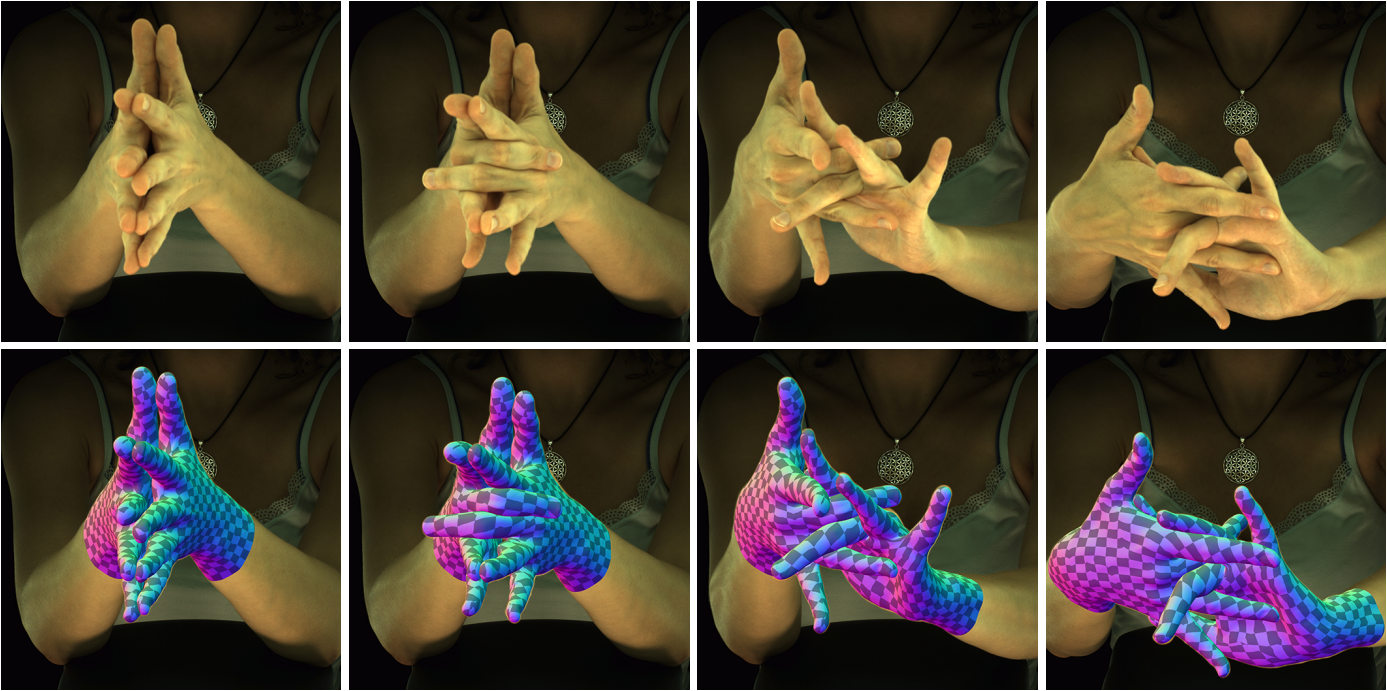
\includegraphics[width=\textwidth]{figures/smithpaper hand tracking.png}
  \caption{Tracking results of method developed by Smith et al. \cite{Smith} of a subjects hands with lots of occlusion and self-contact.}
  \label{fig:smithOcclusion}
\end{figure}


\subsection{Intuitive and comfortable gestures}\label{ergonomics}
For the design of a hand gesture vocabulary, the first consideration might be how well the gesture can be identified. However, gestures that are easily recognized may not be intuitive and easy to perform by the user. According to Stern et al. \cite{Stern2006} there are three factors that should be maximized when choosing a gesture: intuitiveness, comfort and recognition accuracy.

Stern et al. define intuitiveness as the cognitive association between a command or intent and its physical gestural expression. Experiments trying to find universal gestures for a virtual reality environment were also made by Pereira et al. \cite{Pereira2015}. In the experiment, 34 participants were asked to come up with gestures for common HCI tasks like delete, open a menu, copy or paste.
This resulted in over 1300 different gestures for 34 tasks. However, only 84 gestures were chosen by three or more subjects, and some of them were for different tasks. Expecting the user to intuitively guess the same gesture that the developers of the virtual environment intended, therefore, seems unrealistic. Constructing a gesture that requires no introduction or tutorial is therefore also not the goal of this paper.

The research of Ardito et al. \cite{Ardito2014} also supports this. They compare trying to design universal gestures to problems that arose with visual languages in the past. They predict that trying to use the same gesture vocabulary over a range of applications and devices is likely to fail. 


As a measure for comfort, Kölsch et al. propose a method that distinguishes between a pose of some joint or body part and the user compensating using other joints to relieve strain. Compensation for a pose that requires the user's head to be tilted onto its side might be to keep the head upright relative to the body but bend the torso to the side. To find the optimal comfort zone of a posture, Kölsch et al. \cite{Koelsch} measure how users compensate or if they execute the pose without compensating. 

There are also other methods that rely on biomechanical models and physics simulations to measure how comfortable a gesture is, but they are prone to errors \cite{Stern2006}.

Another source of knowledge to tap into regarding gestures is sign language interpreters. They might spend more than 20h per week signing, and they also often suffer from hand pain and fatigue while gesturing for long sessions. This would also be a risk for prolonged sessions in virtual reality that use hand-tracking gestures. Rempel et al. conducted a study with experienced sign language interpreters to find the discomfort level associated with signing selected hand postures, motions and characters \cite{Rempel2014}. 

Rempel et al. \cite{Rempel2014} collected findings and summarized:
\begin{itemize}
  \item Hands should be near the midline of the body and not further apart than the shoulders. They should be near the height of the elbows and close to the lower chest so that the shoulder muscles are not tense. 
  \item Sustained elbow flexion of more than 90 degrees should be avoided.
  \item The most comfortable postures were between neutral and 45 degrees of pronation (palms rotated toward the ground). Repeated full rotations to palm up (supination) or palm down (pronation) should be avoided.
  \item Gestures that included the movement of the elbow or shoulder were more comfortable than gestures with just finger movements.
  \item The more comfortable gesture motions were up-down hand movements performed with motion at the elbows or side-to-side hand movements with motion at the shoulders. 
  \item the most comfortable hand gestures were with the wrists straight and the fingers slightly flexed or in a loose fist.
  \item The least comfortable gestures were those involving wrist flexion, discordant adjacent fingers, or fingers extended.
  \item The position of the thumb did not appear to have a large influence on comfort.
\end{itemize}



\section{Usage in Games}
In the games industry, there are some examples of gesture-based movement present. The gestures used are probably tested and evaluated internally, but there is currently no information published on how well they work and if they are ergonomic or usable. That means that, for now, they can only be compared on the basis of personal experience. 


\subsection{Vacation simulator}
Vacation simulator \cite{VacSimOculus} is a VR simulation game, the sequel to the popular game Job Simulator. Released in 2019 by Owlchemy Labs, it was updated in late 2020 to enable hand-tracking support \cite{VacSimBlog}. The game has a lot of intuitive mechanics that translate very well to hand-tracking, like its use of a physical backpack as a game menu. The teleportation system is very easy to control but comes with the limitations that the user can only teleport to large predefined areas. Therefore, the gesture does not need to be very accurate. The user only needs to "pull" the target closer using a gesture shown in figure \ref{fig:pull}. 

\begin{figure}[hbt!]
  \centering
  \includegraphics[width=\textwidth]{figures/vacsim.jpg}
  \caption{Selecting a target area and confirming teleportation in Vacation Simulator}
  \label{fig:pull}
\end{figure}

This works well for this use case, where the teleportation does not need to be accurate. During testing, this was never a problem and might have even been more intuitive than using a controller because it's so easy to remember and control, whereas some inexperienced users sometimes seem to have problems with the activation of controller-based teleportation using the joystick. 


\subsection{Elixir}
One of the first hand-tracking titles for the Meta Quest was Elixir \cite{Magnopus}. A short demo game where a user is allowed to explore a magic chamber. The chamber could be explored using Room-scale-based movement if the user has a large enough play space. However, there is also a teleportation system included. It works using a bimanual gesture. Both hands form a triangle using both thumbs and index fingers. This can be used to target a point on the floor. The teleport resolution is limited to a grid system on the floor. Once selected, a tile on the floor lights up. To confirm the tile as the target location, the user pinches the respective thumbs and index fingers together. The viewpoint is instantly moved to the new location.

\begin{figure}[hbt!]
  \centering
  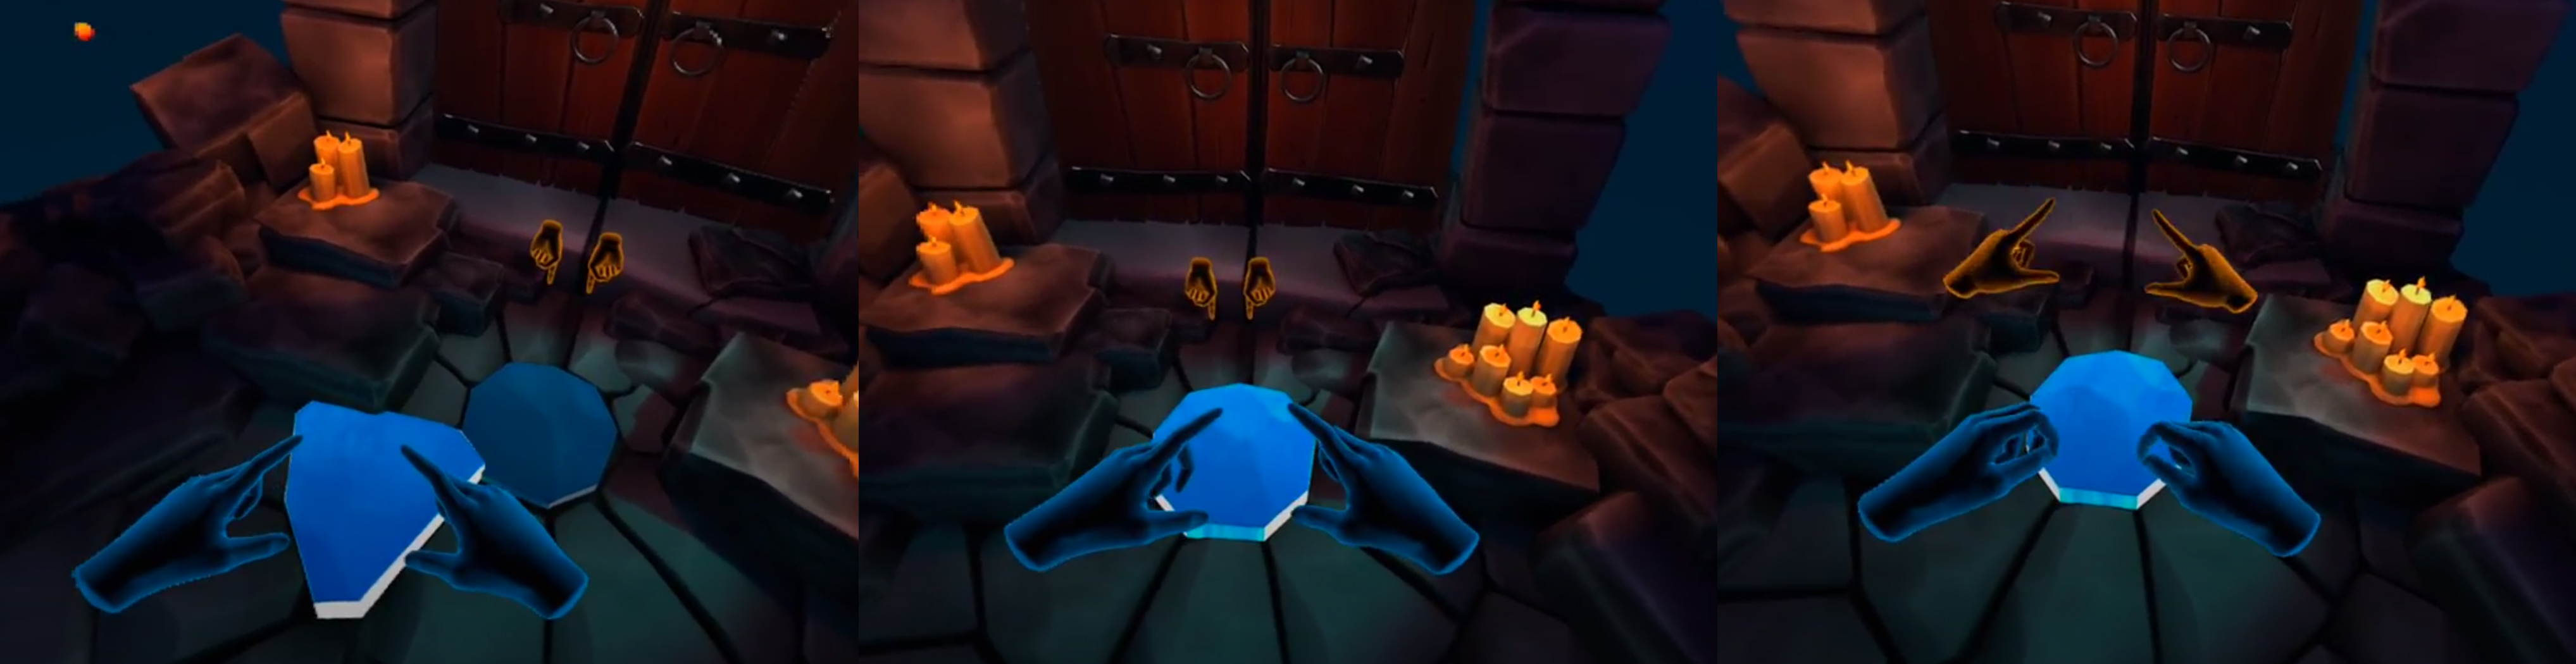
\includegraphics[width=\textwidth]{figures/elixir.jpg}
  \caption{Selecting a target and confirming teleportation in Elixir}
  \label{fig:elixir}
\end{figure}

The system does not allow the user to teleport to any point, which is technically a limitation. However, in practice, it makes the tracking more stable while still allowing good control. Having a gesture to confirm makes the system feel controllable. 


\subsection{Waltz of the Wizard}
In the fantasy game Waltz of the Wizard, \cite{WaWizOculus} by the Studio Aldin Dynamics \cite{Aladin}, the user can learn spells and have fun manipulating the environment. The game has been updated to support hand-tracking \cite{WaWizBlog}. This also includes an adaptation of the custom teleport system the game used in its original version called Telepath \cite{WaWizTelePath}. To move, the user draws a path on the floor. This path is broken up into sections. The system moves the users' viewpoint from one point to the next while dynamically adjusting the pause between the teleport steps. This allows the user to pick up objects while walking or increase the walking speed by swinging arms. In contrast to the other systems, Telepath can be used to move to any point without the limitations of the other systems. It does not require a grid system on the floor and is not limited to only specified teleport points.

\begin{figure}[hbt!]
  \centering
  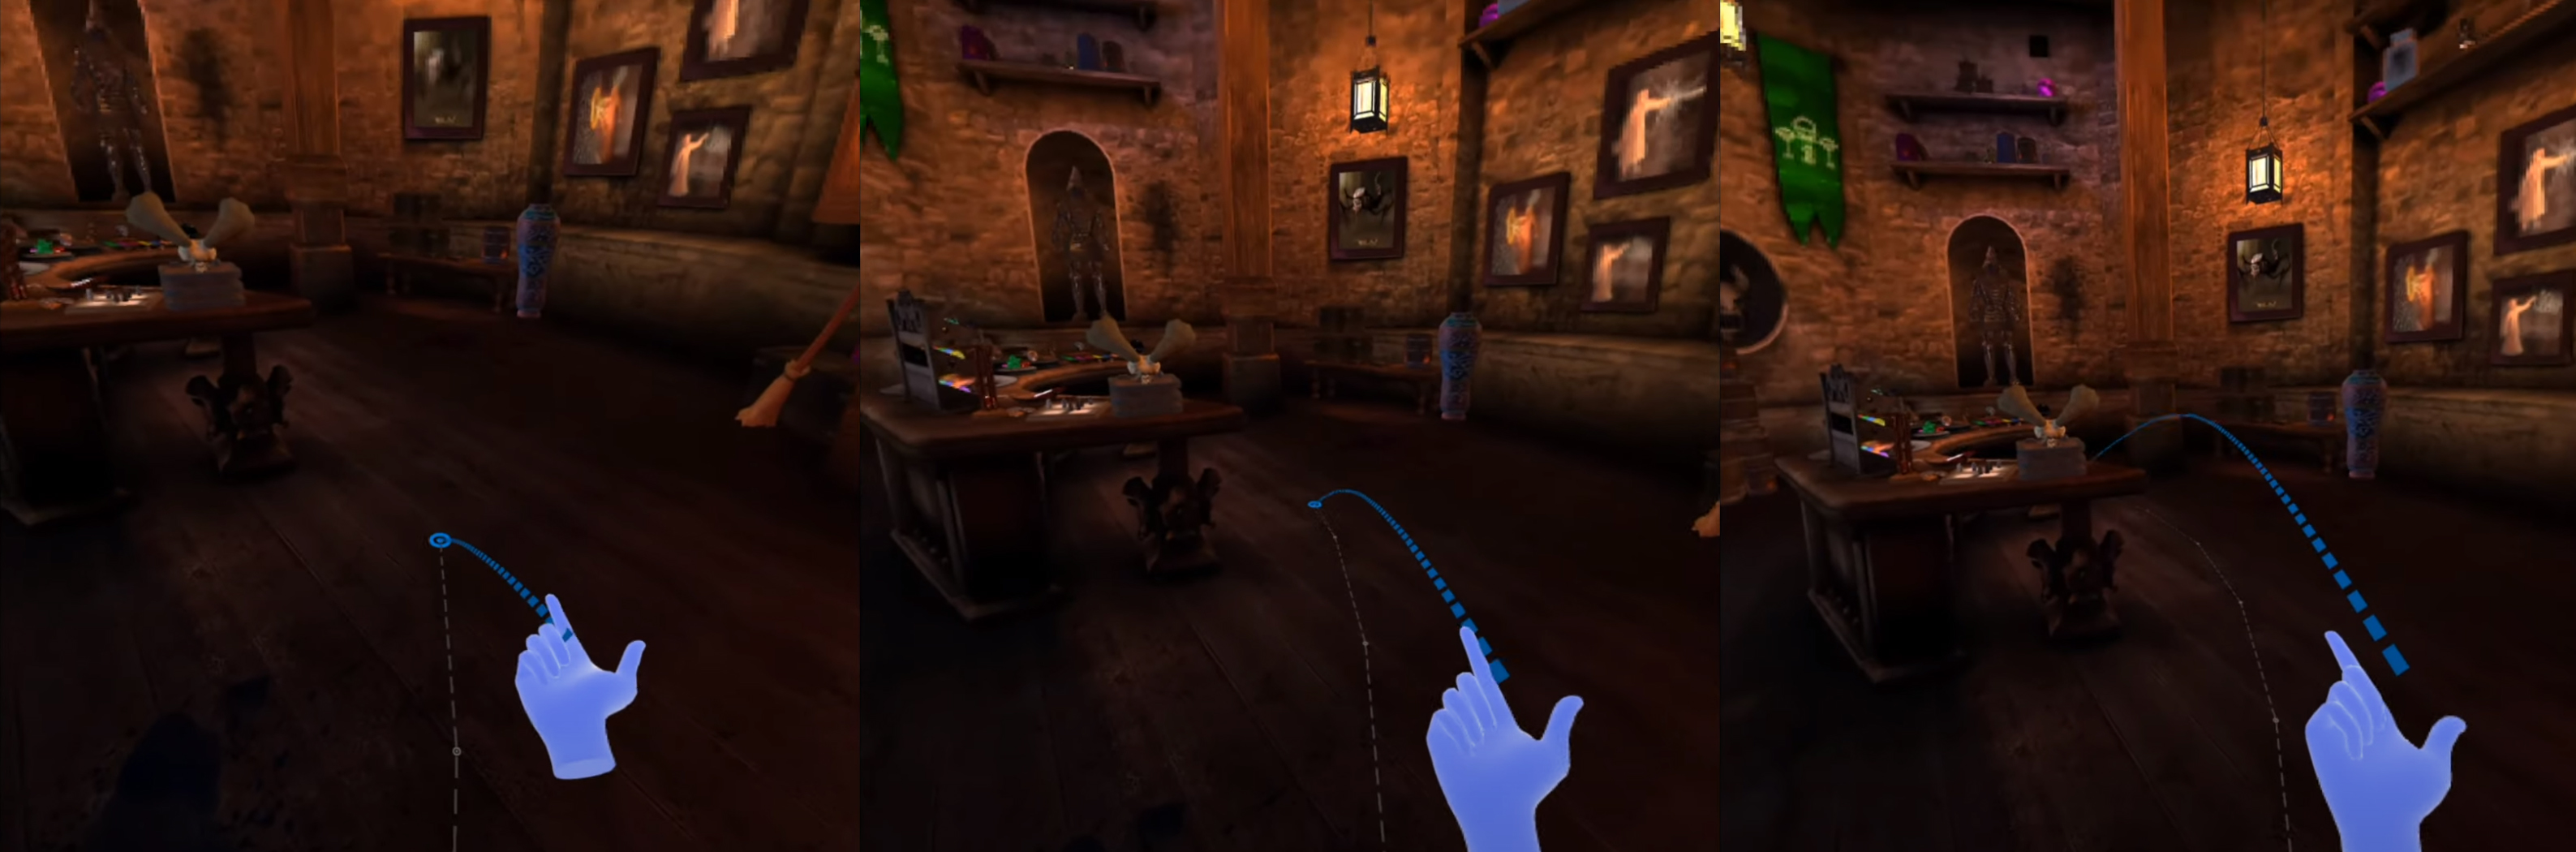
\includegraphics[width=\textwidth]{figures/waltz of the wizard - point.jpg}
  \caption{Telepath gesture: draw walking path using index finger}
  \label{fig:telepath}
\end{figure}

During testing, the Telepath system did not induce cybersickness even though the movement required a short period of getting used to it. The accuracy of the gesture recognition system left a lot to be desired, however, and the experience was frustrating at times. Ergonomics is also a point to criticize since the gesture strains the hands quite uncomfortably even after only a short test of 20 minutes. Drawing a path still seems to be a promising idea and might enable high levels of immersion and allow the brain to perform path integration while not inducing cybersickness. Short bursts of quick movements have also been analyzed by Bhandari et al. \cite{Bhandari}. It produced promising results regarding cybersickness and path integration. 

\section{Study Designs}
For the comparative user study, it is helpful to look at methods used in the literature. 


The study designed by Bozgeyikli et al. \cite{bozgeyikli} compares three locomotion systems in the same environment. A gesture-based point and teleport system, a walk-in place system and a system using a joystick. The latter two are continuous locomotion systems, while the first is a teleportation system. The environment was designed to be very basic to keep the focus on locomotion. It includes six target points with a 0.6m radius placed on the ground. There are also 21 obstacle pillars scattered around the environment. The task for the users is to move to a highlighted target, wait for 3 seconds on the point and then move on to the next point.

The independent variable in this study and all others described here is the gesture tested. The dependent variables are the time to reach destination points, the number of collisions with the obstacles and the results of the usability survey. 
However, collisions can only occur while using the two types of continuous locomotion. 



The study designed by Schäfer et al. \cite{Schafer2021} also uses a primitive environment in the form of a long corridor to reduce the wow effect for first-time users. The environment includes ten markers spaced out along the corridor. The participant's task is to touch all the markers while travelling through the corridor. To explain the gestures, an introduction is added to the study in the form of a tutorial video.

In this case, the dependent variables are the task completion time, the number of teleports, the number of times the tracking is lost and the results of a usability survey.


The study designed by Caggianese et al. \cite{Caggianese} uses a detailed, immersive environment as shown in figure \ref{fig:path}. It includes a very long pathway of 343m with distractors along the way. The user's task is to follow the path from start to end as quickly as possible without going off to the sides.

The dependent variables in this study are the efficiency and effectiveness of each gesture. Efficiency is derived from the task completion time. The effectiveness is derived from performed errors, locomotion interruptions and tracking errors. There are also five standard questionnaires (SSQ, SAM, SUS, SEQ, NASA-TLX) for each participant to fill out after each run.

\begin{figure}[hbt!]
  \centering
  \includegraphics[width=\textwidth]{figures/path-of-study.PNG}
  \caption{Caggianese et al. \cite{Caggianese} Task}
  \label{fig:path}
\end{figure}

Bozgeyikli et al. \cite{bozgeyikli} conducted a study to compare task execution time, but also the accuracy and controllability of different locomotion mechanics. They developed an experiment that took place in a neutral VR environment with 5 checkpoints placed in a pattern. They had participants travel to each checkpoint twice in a fixed order. The participants had to stand on each checkpoint for three seconds to activate the next one. This was implemented to detect accidental movement activations. After six completed checkpoints, obstacles, shown in figure \ref{fig:obstacles}, would be placed in the environment that users should avoid while traveling. The trajectories where recorded to create visualizations like the one shown in figure \ref{fig:pointandTp}.

\begin{figure}[!h]
  \minipage{0.45\textwidth}
      \includegraphics[width=\linewidth]{figures/point&tp.JPG}
      \caption{Visualization of movement trajectories by Bozgeyikli et al. \cite{bozgeyikli}}
      \label{fig:pointandTp}
  \endminipage\hfill
  \minipage{0.45\textwidth}
      \includegraphics[width=\linewidth]{figures/obstacles.JPG}
      \caption{Environment used by Bozgeyikli et al. \cite{bozgeyikli}}
      \label{fig:obstacles}
  \endminipage\hfill
\end{figure}

\section{Conclusion}
The research done so far has not produced a conclusive answer on how to teleport using hand gestures. It is even disputed if such a solution is possible to find at all. The game industry has found some methods for different use cases and environments. There is, however, no way to compare them in a controlled environment since they are each implemented in their respective games. Therefore a flexible test environment is needed to be able to compare gestures in a standardized way. Also none of the developers or authors of the papers describe their approach as user centered or carried out a gesture elicitation study. This makes it hard to argue how intuitive the gestures are to users. This will be addressed in the following chapter. 
